\chapter{Theory and Motivations}
\label{chap:theory}

%\chapterquote{I may not be there yet, but I am closer than I was yesterday}
%{Unknown}

%% Note that the citations in this chapter use the journal and 
%% arXiv keys: I used the SLAC-SPIRES online BibTeX retriever 
%% to build my bibliography. There are also quite a few non-standard
%% macros, which come from my personal collection. You can have them
%% if you want, or I might get round to properly releasing them at 
%% some point myself.

\chapterquote{Absence of evidence is not evidence of absence.}
{Carl Sagan, 1934 - 1996}%


This chapter introduces the \ac{SM} as a gauge invariant \ac{QFT}, and gives a description of the fundamental particles and their interactions.
The shortcomings of the \ac{SM}, outlined in Section~\ref{th:BSM}, imply however that it must be an incomplete description of nature. 
A Supersymmetric extension of the SM can address many of these limitations and is described in Section~\ref{th:SUSY}. 
Particular emphasis is placed on the arguments for \ac{SUSY} with compressed mass spectra in Section~\ref{th:CMPsusy}, as this is the subject of this thesis.
The convention $c=\bar{h}=1$ is used throughout. 
The four vector indices are labelled $\mu$ and $\nu$.
The $SU(2)$ generators are labelled $i$, $j$, and $k$, while the $SU(3)$ generators are labelled $a$, $b$, and $c$.
Gravity, of order $10^{33}$ times weaker than the forces discussed in this chapter, is neglected.
The lack of any explanation of gravity within the \ac{SM} suggests its incompleteness as a total description of nature.

\section{The Standard Model of Particle Physics \label{th:sm}}

The \ac{SM} of particle physics provides a fantastically accurate description of the fundamental particles of nature and their interactions via the strong, electromagnetic, and weak forces at the electroweak energy scale.
It has proved itself incredibly robust during the first years of \ac{LHC} running. 
Many high precision measurements are consistent with their loop level \ac{SM} predictions, see Figure~\ref{fig:stairwayToHeaven}, which shows 
experiment and theory expectations agree over 6 orders of magnitude, across many different processes.
Even very rare processes have been measured to agree with their \ac{SM} predictions: the decay $B_{S}\rightarrow \mu\mu$, very sensitive to new physics processes, has been observed at the level of three in every billion decays of the $B_{S}$ meson~\cite{BSmumuCombo}.
Such tests of the \ac{SM} cement its place as one of the major successes of 20$^{\rm th}$ century physics.


\begin{figure}[htbp]
  \begin{center}
  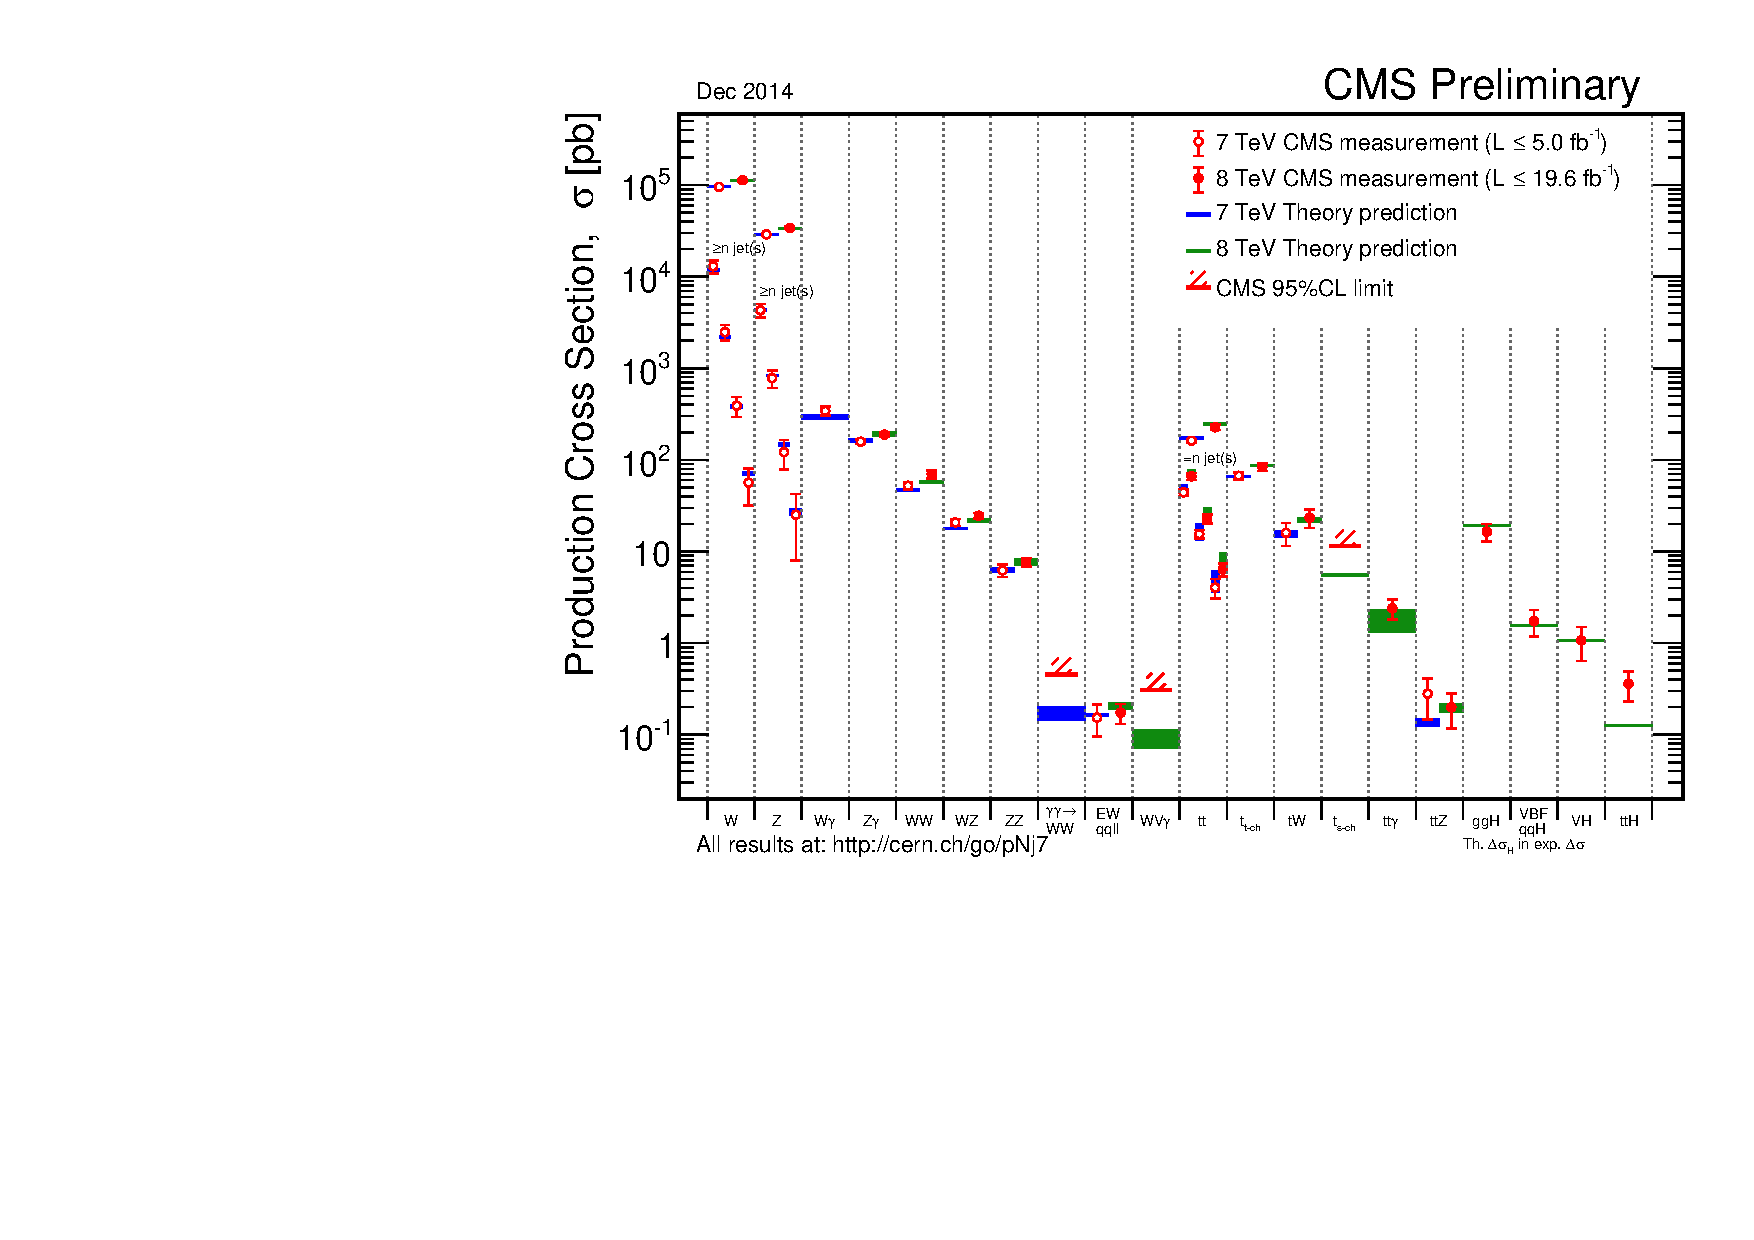
\includegraphics[width=0.8\textwidth]{Figures/theory/SigmaNew_v0}
  \caption{Combined results from \ac{CMS} of many \ac{SM} measurements made at \ac{LHC} centre-of-mass energies of 7 and 8~\TeV, taken from~\cite{CMSpublictwiki}. Theory and experiment agree over a vast range of production cross section values, for many different \ac{SM} processes.
}
  \label{fig:stairwayToHeaven}
  \end{center}
\end{figure}

Developed in the 1960's and 1970's~\cite{PhysRevLett.19.1264,Glashow:1961tr,Salam:1968rm,Hooft1971167}, the \ac{SM} is a relativistic \ac{QFT} in which particles are excitations of fields. 
It is gauge invariant, guaranteeing its renormalizability, and contains three symmetries:
$SU(3)_{C} \times SU(2)_{L} \times U(1)_{Y}$.
$SU(3)$ describes the strong force, felt by coloured particles, 
and $SU(2) \times U(1)$ describes the unified Electromagnetic and Weak forces, felt by particles with weak isospin and weak hypercharge. 
The Higgs mechanism~\cite{PhysRevLett.13.508} describes the spontaneous symmetry breaking of the $SU(2) \times U(1)$ gauge symmetry which allows massive gauge bosons in a gauge invariant way.
The discovery of the Higgs boson~\cite{Aad:2012tfa,Chatrchyan:2012ufa} in July 2012, the mediator of the Higgs field, provided the last piece of the \ac{SM}. 
% Here, the subscript $C$ is for colour charge,
% $L$ is to signify only left handed fermions belong to the group, and $Y$ is for the Yukawa couplings which affect all matter.


\subsection{Fundamental particles and forces}
All known matter in the universe can be described by the fundamental matter particles, which can be separated into quarks - those that feel the strong force, and leptons - those that do not.
Matter particles are all spin-$\frac{1}{2}$ fermions that conform to Fermi statistics and obey the Dirac equation:
%
\begin{eqnarray}
\label{eqn:Dirac}
(i \gamma ^{\mu} \delta_{\mu} - m) \phi =0,
\end{eqnarray}
%
where $\gamma^{\mu}$ are the Dirac matrices, which are defined by their anti-commutation relation 
$\left\{ \gamma^{\mu}, \gamma^{\nu} \right\} = \gamma^{\mu} \gamma^{\nu} + \gamma^{\nu} \gamma^{\mu} = 2 \eta^{\mu\nu}I_{4}$,
where
$ \eta^{\mu\nu} $ is the Minkowski metric $(+, -, -, -)$, and $I_{4}$ is the four-dimensional identity matrix;
$\delta_{\mu}$ is the covariant derivative; and $m$ is the mass of the particle.
Repeated indices are summed over~\cite{HalzenMartin}.

A summary of the matter particles of the \ac{SM} can be found in Table~\ref{tab:SMfermions}. 
A similar table exists for the antiparticles of the leptons and quarks, a consequence of Equation~\ref{eqn:Dirac}, which has both positive and negative energy solutions. 
Rather than particles travelling backwards through time, as the negative energy solutions suggest, anti-particles are interpreted to have all of the same properties as their partner particles but with opposite charge.

%
Leptons are fundamental, free particles in nature. Conversely, quarks are fundamental but not free particles; they form hadrons: baryons, which consist of 3 quarks or anti-quarks, and mesons, a bound quark-anti-quark pair. 
This difference is due to the colour charge that quarks carry: they interact with the strong force, whereas the colourless leptons do not. 

Matter particles interact via the exchange of spin-1 gauge bosons. 
The photon $\gamma$ mediates the electromagnetic interaction and the heavy $\W^{\pm}$ and $\Z$ bosons mediate the weak interaction, through the mixing of the gauge fields when the respective forces are unified. There are 8 colourless gluons ($g$) that mediate the strong force.
The properties of these bosons, and similarly the properties of the interactions, are a direct result of their gauge symmetry groups, detailed in Section~\ref{th:gauge}.
A summary of the bosons can be found in Table~\ref{tab:SMbosons}.
%
%
\begin{table}[h]
\begin{tabular}{c|ccc|ccc}
\hline
\multicolumn{7}{c}{Matter fermions: spin-$\frac{1}{2}$} \\ \hline
 & \multicolumn{3}{c|}{Leptons} &\multicolumn{3}{c}{Quarks} \\ 
Generation & Particle & Mass (MeV) & Charge & Particle & Mass (MeV) & Charge \\ \hline
\multirow{2}{*}{1} & $\nu_{e}$    & 0    & 0  & d & 2.3  &$-\frac{1}{3}$\\
 				   & $e$          & 0.511& -1 & u & 4.8  &$+\frac{2}{3}$\\
\multirow{2}{*}{2} & $\nu_{\mu}$  & 0    & 0  & s & 95   &$-\frac{1}{3}$\\
 				   & $\mu$        & 106  & -1 & c & 1270 &$+\frac{2}{3}$\\
\multirow{2}{*}{3} & $\nu_{\tau}$ & 0    & 0  & b & 4180 &$-\frac{1}{3}$\\
				   & $\tau$ 	  & 1780 & -1 & t & 173000 &+$\frac{2}{3}$\\ \hline
\end{tabular}
\caption{\label{tab:SMfermions}Summary of the particles of the \ac{SM} of particle physics. Fermions, of spin-$\frac{1}{2}$ are shown, split into the three generations of leptons and quarks.}
\end{table}

\begin{table}[h]
\begin{tabular}[h]{c|cccc}	
\hline
\multicolumn{5}{c}{Force carrying gauge bosons: spin-1} \\ \hline
Force & Particle & Symbol & Mass (GeV) & Charge \\ \hline
Electromagnetic & Photon & $\gamma$ & 0 & 0 \\ 
\multirow{3}{*}{Weak} & W boson & $W^{+}$ & 80.4 & 1 \\
& W boson & $\W^{-}$ & 80.4 & -1 \\
& Z boson & $\Z$ & 91.2 & 0 \\
Strong & Gluons (8) & $g$ & 0 & 0 \\ \hline
\multicolumn{5}{c}{Higgs Boson: spin-0} \\ \hline
- & Higgs & $H^{0}$ & 126 & 0 \\ \hline
% & Higgs boson & &&& \\ % $H^{0}$ & 126~\GeV & 0 \\ \hine
\end{tabular}
\caption{\label{tab:SMbosons}Summary of the gauge bosons of the \ac{SM}. The force carrying bosons of spin-1 are shown, with the Higgs boson to complete the picture.}
\end{table}
%
%historical context
%The first generation of leptons were the first to be found. 
The electron was discovered by J.J. Thomson in the Canvendish Laboratory in 1897, and the electron (anti)-neutrino was first proposed by Pauli in 1930 to explain the energy spectrum of beta decay, though it was not discovered until 1956 by Cowan and Reines at Los Alamos~\cite{CowanReines}.
The muon was discovered in 1936 by Anderson and Neddermeyer at Caltech in studies of cosmic rays, and confirmed a year later in a cloud chamber experiment.
The muon neutrino was then discovered in 1962 by Lederman, Schwartz and Steinberger, after being proposed in the early 1940s.
The $u$, $d$, and $s$ quarks were first proposed in 1964 by Gell-Man and Zweig to explain the  `Eightfold' hadron structure~\cite{GellMann:1964nj,Zweig:1964jf},
and the three quarks were observed in deep inelastic scattering experiments at the \ac{SLAC} 4 years later.
The proposal of the GIM mechanism~\cite{PhysRevD.2.1285} in 1970 predicted the completion of the second generation - the charm quark in order to explain the observed suppression of \ac{FCNC}s. 
%
The third generation was more of a surprise - the $\tau$ lepton was proposed to explain an excess of events at the $e^{+}e^{-}$ colliding ring at \ac{SLAC} in the mid 1970's, and the $\nu_\tau$ was not discovered until 2000, completing the lepton family. 
CP violation in kaon decay drove the proposal of the third quark generation in 1973~\cite{Kobayashi01021973}.
The bottom quark was first observed in 1977 at Fermilab with the obervation of bottomium. 
The top quark, after years of dedicated searches, was not discovered until 1995 at the Tevatron.

%
The \ac{SM} was thus built as a theory over several decades; driven by the need to explain experimental observations, and predicting the existence of particles that were then found later after dedicated searches. 
%bosons%


\subsection{Gauge Symmetries \label{th:gauge}}

\subsection{Electroweak Symmetry Breaking and the Higgs\label{th:EW}}

\section{Motivation for Physics Beyond the Standard Model \label{th:BSM}}

\section{Supersymmetry \label{th:SUSY}}

\subsection{Compressed Supersymmetry \label{th:CMPsusy}}

